% !TeX encoding = UTF-8
% !TeX spellcheck = en_US
\documentclass[title={Introduction to R}, author={Mutschler and Zaharieva}, inst={Institute for Econometrics and Empirical Economics}]{beamer}
\usepackage{lmodern}
\usepackage[utf8]{inputenc}
\usepackage[T1]{fontenc}
\graphicspath{{graphics/}}
\begin{document}

\title[Introduction to R]{Introduction to R}
\author[ \ ]{Dr.\ Willi Mutschler \\ \vspace{0.5cm} Dr.\ Martina Danielova Zaharieva}
\date{Summer 2018}
\institute[CQE]{\ }
\maketitle

\section{General information}

\begin{frame}
\frametitle{General information}
\framesubtitle{Aims and prerequisites}
\begin{itemize}
\item Objective: Learn how to use R for econometrics and statistics
\item Prerequisites:
\begin{enumerate}
\item Basics in probability theory and statistical inference\newline
(Mosler and Schmid, Wahrscheinlichkeitsrechnung und schlie\ss ende
Statistik, 2008)
\item Multiple linear regression\newline
(von Auer, \"{O}konometrie, 2011)
\end{enumerate}
\item Laptop (any standard operating system), \newline
if possible with Wifi internet access
\end{itemize}
\end{frame}


\begin{frame}
\frametitle{General information}
\framesubtitle{Literature}
\begin{description}
\item[Essential:] Andreas Behr and Ulrich P\"{o}tter%
\newline
\emph{Einf\"{u}hrung in die Statistik mit R}\newline
2. Aufl., Vahlen: 2011.\medskip
\item[Additional:] W.N. Venables and B.D. Ripley\newline
\emph{Modern Applied Statistics with S}, 4th ed., 2002.\smallskip
\item Grant V. Farnsworth, \emph{Econometrics in R}, 2008 (pdf).\smallskip
\item Phil Spector, \emph{Data Manipulation with R}, 2008.\smallskip
\item Paul Murrell, \emph{R Graphics}, 2006.
\end{description}
\end{frame}


\begin{frame}
\frametitle{General information}
\framesubtitle{Schedule (I)}
\begin{enumerate}
\item Introduction, installation, editor, help, packages
\item Operators and functions
\item Data import and export
\item Indexing
\item User-defined functions
\item Sorting and merging
\item Data description (univariate and multivariate)
\item Random numbers and simulations
\item Linear regressions
\item Numerical optimization
\item Maximum likelihood estimation
\item Advanced graphics
\end{enumerate}
\end{frame}


\begin{frame}
\frametitle{General information}
\framesubtitle{Schedule (II)}
Optional additional topics:
\begin{itemize}
\item date and time information
\item time series
\item wishes?
\item \ldots
\end{itemize}
\end{frame}


\begin{frame}
\frametitle{General information}
\framesubtitle{Final Exam}
\begin{itemize}
	\item The exam consists of assignments you have to solve at home
	\item We will hand out the exam on Friday April 6 10 am
	\item Deadline to hand in your solutions: Friday April 13, 10 am
	\item Important: Do not forget to register with the Prüfungsamt for ''Vorgezogene Prüfung''
	\item We will NOT communicate grades before the beginning of May (after it is not possible anymore to resign your official registration for the course)
	
\end{itemize}

\end{frame}


\section{Introduction}

\begin{frame}
\frametitle{Introduction}
\framesubtitle{About R}
\begin{itemize}
\item S is an object-oriented statistical computing language
\item The language S is implemented as S-Plus (commercial) \newline
and R (OpenSource)
\item The differences between S-Plus and R are minimal
\item Similar programming languages: Matlab, GAUSS, Julia
\item R is available for Windows, Linux and MacOS
\item Internet site: \texttt{www.r-project.org}
\item Comprehensive R Archive Network : \texttt{cran.at.r-project.org}
\end{itemize}
\end{frame}


\begin{frame}
\frametitle{Introduction}
\framesubtitle{Installation (for Windows)}
\begin{itemize}
\item Open \texttt{www.r-project.org} in your browser
\item In the left menu, choose CRAN (or click \textquotedblleft download
R\textquotedblright )
\item Choose a mirror (e.g. Germany)
\item Choose you operating system (e.g. Windows)
\item Choose \texttt{base}
\item Download the newest version of R
\item Execute \texttt{R-3.4.x-win.exe} and follow the instructions
\item Start R
\end{itemize}
\end{frame}


\begin{frame}
\frametitle{Introduction}
\framesubtitle{Command window}
Command window (R Console)
Prompt: \texttt{>}
You can input commands and execute them \newline
(by pressing the \textsc{Return} key)
\begin{block}{Examples}
\texttt{> 1+1}\newline
\texttt{> 1+1 \# This is a comment: 1+1}\newline
\texttt{> (1+2)*3}\newline
\texttt{> (5/3)\symbol{94}4.5}\newline
\texttt{> 5+2; 7+3; 2*5}
\end{block}
\end{frame}


\begin{frame}
\frametitle{Introduction}
\framesubtitle{Command window}
Concatenation: \texttt{c()}
Assignment operator: \texttt{<-} or \texttt{=}
\begin{block}{Examples}
\texttt{> c(1,4,7)}\newline
\texttt{> a <- c(1,4,7)}\newline
\texttt{> print(a)}\newline
\texttt{> a}\newline
\texttt{> A}\newline
\texttt{> b <- c(1,a,3)}\newline
\texttt{> b}\newline
\texttt{> mean(b)}
\end{block}
\end{frame}


\begin{frame}
\frametitle{Introduction}
\framesubtitle{Command window}
Quitting
\begin{itemize}
\item Quit R by the command \texttt{q()}
\item In general, do \emph{not }save your workspace
\end{itemize}
\end{frame}


\begin{frame}
	\frametitle{Introduction}
	\framesubtitle{Style Guide}
	\begin{itemize}
		\item Variable names and commands are case-sensitive		
		\item Names may include letters, numbers, dots		
		\item Use a consistent style (e.g Google's R style guide or at least the recommendations of the next slides, based on "Advanced R" by Hadley Wickham)
	\end{itemize}
\end{frame}


\begin{frame}
	\frametitle{Introduction}	
	\framesubtitle{Style Guide}	
	\begin{itemize}
		\item File names should be meaningful and end in .R
		\item Variable and function names should be lowercase. Use an underscore to separate words within a name. Generally, variable names should be nouns and function names should be verbs. Strive for names that are concise and meaningful (this is not easy!). 
		\item Avoid using names of existing functions and variables.
		\item Place spaces around all infix operators (=, +, -, $<$-, etc.).
		\item Always put a space after a comma, and never before (just like in regular English).
	\end{itemize}
\end{frame}


\begin{frame}	
	\frametitle{Introduction}	
	\framesubtitle{Style Guide}	
	\begin{itemize}
		\item Do not place spaces around code in parentheses or square brackets (unless there’s a comma).
		\item An opening curly brace should never go on its own line and should always be followed by a new line. A closing curly brace should always go on its own line, unless it’s followed by else.
		\item Strive to limit your code to 80 characters per line.
		\item Use $<$-, not =, for assignment. 
		\item Comment your code. Each line of a comment should begin with the comment symbol and a single space: $\#$. Comments should explain the why, not the what. 
	\end{itemize}
\end{frame}


\begin{frame}
\frametitle{Introduction}
\framesubtitle{Editors}
\begin{itemize}
\item Long computations should not be done interactively in the command
window
\item Use an editor to write a program and then execute it in R
\item There is a built-in editor in R: Datei -- Neues Skript
\item External editors:
\begin{itemize}
\item R-Studio, \texttt{http://www.rstudio.com/ide/download/}
\item Tinn-R, \texttt{http://sciviews.org/Tinn-R/}
\item Notepad++: \texttt{http://www.notepad-plus-plus.org/}
\end{itemize}
\end{itemize}
\end{frame}


\begin{frame}
\frametitle{Introduction}
\framesubtitle{Internal editor}
\begin{itemize}
\item Open a new script
\item Type a few lines of commands, e.g.\newline
\texttt{a <- c(1,4,7)}\newline
\texttt{mean(a)}\newline
\texttt{mean(a)\symbol{94}2}
\item Execute a single line by pressing \textsc{Ctrl-R}
\item Execute multiple lines by marking them and then pressing \textsc{Ctrl-R} or \textsc{Ctrl-Return}
\item Save the script, quit R, restart R, open the script and execute it
\end{itemize}
\end{frame}


\begin{frame}
\frametitle{Introduction}
\framesubtitle{Help etc.}
\begin{itemize}
\item To obtain details about a command, type \newline
\texttt{?command} \newline
or \newline
\texttt{help(command)}
\item Example: \texttt{?mean} or \texttt{help(mean)}
\item Start the \textquotedblleft help center\textquotedblright : \texttt{help.start()}
\item Task Views on CRAN
\item R Journal on CRAN
\end{itemize}
\end{frame}


\begin{frame}
\frametitle{Introduction}
\framesubtitle{Packages}
\begin{itemize}
\item One of the strengths of R is the large and growing collection of packages that can be downloaded from CRAN (or installed off-line)
\item Online installation: Pakete --- Installiere Paket(e)\ldots
\item Offline installation: \texttt{install.packages(''packagename'')}
\item Installed packages are activated by \texttt{library(packagename)}
\item Help about packages: \texttt{library(help=packagename)}
\item Install, activate and look into the help of the package MASS
\end{itemize}
\end{frame}


\begin{frame}
\frametitle{Introduction}
\framesubtitle{R objects}
\begin{itemize}
\item R is object oriented
\item An object can be anything: scalar, vector, matrix, string, table, factor, list, data frame, regression results, \ldots
\item The object type determines how some commands work \newline
(e.g. \texttt{plot}, \texttt{summary})
\item Every object has a unique name
\item List of all objects: \texttt{ls()}
\item Delete (\textbf{r}e\textbf{m}ove) objects: \texttt{rm()}
\end{itemize}
\end{frame}


\begin{frame}
\frametitle{Introduction}
\framesubtitle{R objects}
\begin{block}{Examples}
\texttt{> x <- c("A","B","C")}\newline
\texttt{> class(x)}\newline
\texttt{> y <- c(1,2,5)}\newline
\texttt{> class(y)}\newline
\texttt{> ls()}\newline
\texttt{> rm(x)}\newline
\texttt{> ls()}
\end{block}\pause
$\longrightarrow $ \textsc{Exercise 1}
\end{frame}


\section{Operators and functions}

\begin{frame}
\frametitle{Operators and functions}
\framesubtitle{Logical operators}
\begin{description}
\item[\texttt{\&}] and
\item[\texttt{|}] or
\item[\texttt{!}] not
\item[\texttt{NA}] no answer (or: not available)
\item[\texttt{==}] equal (do \emph{not} use \texttt{=})
\item[\texttt{>}, \texttt{>=}] greater than,
greater than or equal
\item[\texttt{<}, \texttt{<=}] less than, less
than or equal
\item[\texttt{!=}] not equal
\end{description}
\end{frame}


\begin{frame}
\frametitle{Operators and functions}
\framesubtitle{Logical operators}
\begin{block}{Examples}
\texttt{5 < 7}\newline
\texttt{1+1 == 3}\newline
\texttt{a <- c(-1,4,9)}\newline
\texttt{a >= 2 \& a < 8}\newline
\texttt{b <- c(NA,1,2,3)}\newline
\texttt{b > 0}\newline
\texttt{is.na(b)}\newline
%\texttt{a[a>2]}\newline
\texttt{a == 4}\newline
\texttt{a = 4}
\end{block}\pause
$\longrightarrow $ \textsc{Exercise 2}
\end{frame}


\begin{frame}
\frametitle{Operators and functions}
\framesubtitle{Arithmetic operators and mathematical functions}
\begin{description}
\item[\texttt{+}, \texttt{-}] plus, minus
\item[\texttt{*}, \texttt{/}] multiplication and division
\item[\texttt{\symbol{94}}] power (exponentiation)
\item[\texttt{Inf}, \texttt{-Inf}] infinity (plus or minus)
\item[\texttt{NaN}] not a number
\item[\texttt{abs}] absolute value
\item[\texttt{sqrt}] square root
\item[\texttt{exp,log}] exponential function and natural logarithm (\emph{not} \texttt{ln})
\item[\texttt{sin}] sinus (other trigonometric functions as well)
\item[\texttt{sum}] sum
\end{description}
\end{frame}


\begin{frame}
\frametitle{Operators and functions}
\framesubtitle{Arithmetic operators and mathematical functions}
\begin{block}{Examples}
\texttt{x <- c(-1,0,2,9,3)}\newline
\texttt{abs(x)}\newline
\texttt{sqrt(x)}\newline
\texttt{1/x}\newline
\texttt{-1/x}\newline
\texttt{0/x}\newline
\texttt{log(x)}\newline
\texttt{x\symbol{94}c(2,3,2,3,2)}\newline
\texttt{x\symbol{94}c(2,3)}\newline
\texttt{log(x)<0}
\end{block}\pause
$\longrightarrow $ \textsc{Exercise 3}
\end{frame}


\begin{frame}
\frametitle{Operators and functions}
\framesubtitle{Matrix functions}
\begin{description}
\item[\texttt{matrix}] creates a matrix from a vector
\item[\texttt{dim}] dimensions of a matrix
\item[\texttt{t}] transpose
\item[\texttt{\%*\%}] matrix multiplication
\item[\texttt{det}] determinant
\item[\texttt{solve}] inverse
\item[\texttt{eigen}] eigenvalues and eigenvectors
\item[\texttt{diag}] diagonal
\item[\texttt{cbind}] merge matrices column-wise
\item[\texttt{rbind}] merge matrices row-wise
\end{description}
\end{frame}


\begin{frame}
\frametitle{Operators and functions}
\framesubtitle{Matrix functions}
\begin{block}{Examples}
\texttt{x <- matrix(c(2,3,4,5,1,1,9,3,2),3,3)}\newline
\texttt{dim(x)}\newline
\texttt{det(x)}\newline
\texttt{solve(t(x)\%*\%x)}\newline
\texttt{x\%*\%c(8,5,1)}\newline
\texttt{diag(x)}\newline
\texttt{diag(x) <- 0}\newline
\texttt{solve(x)\%*\%x}\newline
\texttt{matrix(NA,4,4)}\newline
\texttt{rbind(cbind(x,x),c(0,1))}
\end{block}\pause
$\longrightarrow $ \textsc{Exercise 4}
\end{frame}


\begin{frame}
\frametitle{Operators and functions}
\framesubtitle{Set operations and special functions}
\begin{description}
\item[\texttt{unique}] the set of all unique elements of a vector
\item[\texttt{union}] $x\cup y$
\item[\texttt{intersect}] $x\cap y$
\item[\texttt{setdiff}] $x\backslash y$
\item[\texttt{\%in\%}] $x\in y$
\item[\texttt{sort}] sort the elements of a vector
\item[\texttt{cumsum}] cumulated sum of a vector \newline
(also \texttt{cumprod}, \texttt{cummin}, \texttt{cummax})
\item[\texttt{which.min}] find the index of the smallest vector element 
\newline
(also \texttt{which.max})
\end{description}\pause
$\longrightarrow $ \textsc{Exercise 5}
\end{frame}


\begin{frame}
\frametitle{Operators and functions}
\framesubtitle{Sequences and replications}
\begin{description}
\item[\texttt{seq}] sequence from $a$ to $b$ of length $n$, \newline
\texttt{seq(from=a,to=b,length=n)}, \newline
or by increments of size $d,$ \newline
\texttt{seq(from=a,to=b,by=d)}
\item[\texttt{a:b}] integer sequence from $a$ to $b$
\item[\texttt{rep}] replicate a vector $n$ times\newline
\texttt{rep(what,times=n)},\newline
or each element $n$ times,\newline
\texttt{rep(what,each=n)}
\end{description}\pause
$\longrightarrow $ \textsc{Exercise 6}
\end{frame}


\begin{frame}
\frametitle{Operators and functions}
\framesubtitle{The apply command}
\begin{itemize}
\item The \texttt{apply} command is very R specific and powerful, but it takes some time to get used to it
\item The general syntax is
\end{itemize}
\begin{center}
\texttt{apply(X, MARGIN, FUN, ...)}
\end{center}

\begin{itemize}
\item The function \texttt{FUN} is applied to all rows (\texttt{MARGIN=1})
or all columns (\texttt{MARGIN=2}) of \texttt{X}
\item All function returns are collected in a vector if they are univariat,
or in a matrix if they are multivariat
\item There are some variants of \texttt{apply} (\texttt{sapply, lapply)}
\end{itemize}
\end{frame}


\begin{frame}
\frametitle{Operators and functions}
\framesubtitle{The apply command}
\begin{block}{Examples}
\texttt{x <- matrix(c(2,3,4,5,1,1,9,3,2),3,3)}\newline
\texttt{apply(x,1,sum)}\newline
\texttt{apply(x,2,sum)}\newline
\texttt{apply(x,2,quantile,prob=c(0.1,0.9))}\newline
\texttt{apply(x,2,function(z) z\symbol{94}2)}\newline
\texttt{apply(x,2,rep,each=2)}\newline
\texttt{apply(x,1,rep,each=2)}
\end{block}\pause
$\longrightarrow $ \textsc{Exercise 7}
\end{frame}


\section{Data import and export}
\begin{frame}
\frametitle{Data import and export}
\framesubtitle{General remarks}
\begin{itemize}
\item R is all about working with data
\item There are various ways to read data from different sources in many
formats
\item In R, datasets are usually represented as \texttt{data.frame} objects
\item The structure of dataframes is similar to matrices
\item Each column is a variable, each row is an observation
\item R has a large collection of \textquotedblleft standard
datasets\textquotedblright , see \texttt{data()}
\end{itemize}
\end{frame}

\begin{frame}
\frametitle{Data import and export}
\framesubtitle{Manual data input}
\begin{itemize}
\item Very small datasets can be typed in directly, e.g.\newline
\texttt{x <- data.frame(v1=c(2,6,1,1),v2=c(9,9,8,8))}
\item To edit existing objects, use \texttt{data.entry}, e.g.\newline
\texttt{y <- data.entry(x)}
\item However, editing data within R is \emph{not} recommended
\item Datasets should be stored outside R, preferably in separate directories
\item The datasets should be easily accessible by data-managing programs
(e.g. Excel, Stata, ASCII editors, \ldots )
\end{itemize}
\end{frame}

\begin{frame}
\frametitle{Data import and export}
\framesubtitle{Saving and loading R objects}
\begin{itemize}
\item All R objects can be saved by the command\newline
\texttt{save(obj1,obj2,...,file="c:/path/name.Rdata")}
\item In principle, other file name extensions are possible, \newline
but not recommended
\item All objects saved in a file can be loaded by the command\newline
\texttt{load("c:/path/name.Rdata")}
\item The data format is R specific and cannot even be read \newline
by S-Plus
\end{itemize}
\end{frame}

\begin{frame}
\frametitle{Data import and export}
\framesubtitle{Reading and writing text files}
\begin{itemize}
\item A convenient command to read simple text files is \newline
\texttt{read.csv("c:/path/filename.txt")}
\item The command assumes the following data format:
\begin{enumerate}
\item The first row contains the variables names, delimited by commas
\item The following rows are the observations, the variables are again
delimited by commas
\item The decimal sign is a dot (not a comma)
\end{enumerate}
\item Use \texttt{read.csv2} if the variables are delimited by semi-colons
and the decimal sign is a comma (i.e. German style)
\end{itemize}
\end{frame}

\begin{frame}
\frametitle{Data import and export}
\framesubtitle{Reading and writing text files}
\begin{itemize}
\item More options are available for the command \texttt{read.table}
\item If the dataset is very large, reading a dataframe may be rather time
consuming
\item You can use the faster (but less convenient) command \texttt{scan}
\item Exporting text files from R is usually not necessary. If it is, use 
\texttt{write.csv}, \texttt{write.csv2} or \texttt{write.table}
\end{itemize}\pause
$\longrightarrow $ \textsc{Exercise 8}
\end{frame}
\begin{frame}


\frametitle{Data import and export}
\framesubtitle{Other data formats}
\begin{itemize}
\item There are many packages that provide easy access to datasets in other
data formats
\item The \texttt{foreign} package includes commands to read the following
formats: \texttt{dbf}, \texttt{Stata}, \texttt{SPSS}, \texttt{SAS}, and a
few more (but not Excel)
\item Excel sheets can be read using the command \texttt{read\_excel} provided
by the package \texttt{readxl}
\item It is possible to access SQL data using the ODBC interface package 
\texttt{RODBC} or \texttt{dplyr}(we skip that)
\end{itemize}
\end{frame}

\begin{frame}
\frametitle{Data import and export}
\framesubtitle{Reading data online}
\begin{itemize}
\item If the data file is located on a server one can simply specify the 
\texttt{url} instead of the file name
\item Zipped files can be unzipped by \texttt{unzip}
\item Some packages (e.g. \texttt{TTR} and \texttt{fImport}) provide
downloading options for financial data
\end{itemize}
\begin{block}{Examples}
\texttt{x1 <- read.csv("http://www....//bsp1.txt")}
\texttt{library(TTR)}
\texttt{y <-getYahooData("IBM")}
\end{block}\pause
$\longrightarrow $ \textsc{Exercise 9}
\end{frame}


\section{Indexing}

\begin{frame}
\frametitle{Indexing}
\framesubtitle{Indexing vectors}
\begin{itemize}
\item R has a rich indexing syntax
\item The basic ideas are the same for vectors, matrices and other objects
\item Indexing is used to read or manipulate specified elements of the
objects
\item Indexes are always given in square brackets: \texttt{[]} \newline
(or sometimes \texttt{[[]]})
\item Indexes can be either numerical or logical
\item We will start with vectors and then look at matrices and dataframes
\item The symbols \texttt{i} and \texttt{j} denote integer variables (not
vectors)
\end{itemize}
\end{frame}


\begin{frame}
\frametitle{Indexing}
\framesubtitle{Indexing vectors}
Numerical indexing
\begin{description}
\item[{\texttt{x[1]}}] first element
\item[{\texttt{x[2]}}] second element
\item[{\texttt{x[i]}}] $i$-th element
\item[{\texttt{x[-i]}}] all elements, without position $i$
\item[{\texttt{x[a:b]}}] all elements from position $a$ to position $b$
\item[{\texttt{x[k]}}] \texttt{k} numerical vector: all elements at positions
given in $k$
\end{description}

Logical indexing
\begin{description}
\item[{\texttt{x[a]}}] \texttt{a} logical vector: all elements where $a$ is
true \newline
(\texttt{a} must have the same length as \texttt{x})
\end{description}
\end{frame}


\begin{frame}
\frametitle{Indexing}
\framesubtitle{Indexing vectors}
\begin{block}{Examples}
\texttt{x <- c(2,3,4,5,1,1,9,3,2)}\newline
\texttt{x[2]}\newline
\texttt{x[4:7]}\newline
\texttt{x[20]}\newline
\texttt{x[-9]}\newline
\texttt{x[-3]}\newline
\texttt{x[c(1,5,1,9,9)]}\newline
\texttt{a <- (x<4)}\newline
\texttt{x[a]}\newline
\texttt{x[x<4]}
\end{block}\pause
$\longrightarrow $ \textsc{Exercise 10}
\end{frame}


\begin{frame}
\frametitle{Indexing}
\framesubtitle{Indexing matrices}
Numerical indexing
\begin{description}
\item[{\texttt{x[i,j]}}] element in row $i$, column $j$
\item[{\texttt{x[,j]}}] column $j$ (as a vector)
\item[{\texttt{x[i,]}}] row $i$ (as a vector)
\item[{\texttt{x[,-j]}}] without column $j$
\item[{\texttt{x[-i,]}}] without row $i$
\item[{\texttt{x[a:b,j]}}] elements $a$ to $b$ in column $j$
\item[{\texttt{x[k,m]}}] \texttt{k},\texttt{m} numerical vectors: all
elements at positions \newline
given in $k$ and $m$
\end{description}
\end{frame}


\begin{frame}
\frametitle{Indexing}
\framesubtitle{Indexing matrices}
Logical indexing
Let \texttt{a} denote a logical matrix of the same dimension as \texttt{x}; 
\newline
let \texttt{k} and \texttt{m} denote logical vectors of suitable length
\begin{description}
\item[{\texttt{x[a]}}] All elements of \texttt{x} at positions where \texttt{a%
} is true, \newline
as a \emph{vector!}
\item[{\texttt{x[,m]}}] All columns of \texttt{x} where \texttt{m} is true
\item[{\texttt{x[k,]}}] All rows of \texttt{x} where \texttt{k} is true
\end{description}
Of course, one may use numerical indexing for one dimension \newline
and logical indexing for the other dimension
\begin{description}
\item[{\texttt{x[k,1:2]}}] All elements of columns 1 and 2 where \texttt{k}
is true
\item[{\texttt{x[3,m]}}] All elements of row 3 where \texttt{m} is true
\end{description}
\end{frame}


\begin{frame}
\frametitle{Indexing}
\framesubtitle{Indexing matrices}
\begin{block}{Examples}
\texttt{x <- matrix(1:16,4,4)}\newline
\texttt{x[3,3]}\newline
\texttt{x[,4]}\newline
\texttt{x[2,]}\newline
\texttt{x[,-1]}\newline
\texttt{x[-3,]}\newline
\texttt{x[2:4,4]}\newline
\texttt{x[c(1,4,2,2,2),1:2]}\newline
\end{block}
\end{frame}


\begin{frame}
\frametitle{Indexing}
\framesubtitle{Indexing matrices}
\begin{block}{Examples}
\texttt{x <- matrix((-7:8)\symbol{94}2,4,4)}\newline
\texttt{a <- (x<10)}\newline
\texttt{x[a]}\newline
\texttt{x[,c(TRUE,FALSE,TRUE,FALSE)]}\newline
\texttt{x[x[,1]<30,3:4]}\newline
\texttt{x[x[,2]==1 | x[,3]==1,]}\newline
\texttt{x[2:4,4]}\newline
\texttt{x[c(1,4,2,2,2),1:2]}
\end{block}\pause
$\longrightarrow $ \textsc{Exercise 11}
\end{frame}


\begin{frame}
\frametitle{Indexing}
\framesubtitle{Indexing dataframes}
\begin{itemize}
\item Dataframes have the same index methods as matrices
\item Logical conditions can include strings (character variables)
\item There are three additional ways to extract dataframe columns:
\begin{enumerate}
\item \texttt{x\$varname}
\item \texttt{x[[i]]} \newline
where \texttt{i} can also be a numerical vector
\item \texttt{x["varname"]} \newline
or \texttt{x[c("varname1","varname2",...)]}
\end{enumerate}
\item Dataframe variables can be addressed directly by their name when you 
\texttt{attach} the dataframe, e.g. \texttt{attach(x)}
\end{itemize}\pause
$\longrightarrow $ \textsc{Exercise 12}
\end{frame}


\section{User-defined functions} 
\begin{frame}
\frametitle{Functions}
\framesubtitle{User-defined functions}
\begin{itemize}
\item One can define new functions in R
\item Functions are objects of class \texttt{function}
\item Each function has a name, one or more inputs (arguments) \newline
and one output (return)
\item Inputs can be any objects (usually vectors)
\item The function can return only one object (which can be a list)
\item Variables defined within a function are only local
\end{itemize}
\end{frame}


\begin{frame}
\frametitle{Functions}
\framesubtitle{User-defined functions}
Syntax\medskip

\texttt{fn <- function(x,y)\{}

\quad \texttt{block of commands to compute output out}

\quad \texttt{return(out)}

\quad \texttt{\}\bigskip}
\begin{block}{Example}
\texttt{utility <- function(cons,gam)\{}

\quad \texttt{U <- (cons\symbol{94}(1-gam)-1)/(1-gam)}

\quad \texttt{return(U)}

\quad \texttt{\}}
\end{block}\pause
$\longrightarrow $ \textsc{Exercise 13}
\end{frame}


\begin{frame}
\frametitle{Functions}
\framesubtitle{More on function arguments}
\begin{itemize}
\item Each arguments of a function must have a unique name
\item When calling a function, the order of the arguments is \newline
arbitrary, if the argument names are explicitly used, \newline
e.g. \texttt{fn(x=5,y=9)} or \texttt{fn(y=9,x=5)}
\item Without argument names, R assigns the values in the order of the
function definition
\item A function definition may include default values for arguments, 
\newline
e.g. \texttt{fn <- function(x,y=1)\{...\}}
\item If an argument with a default value is missing in a function call, R
uses the default value
\end{itemize}
\end{frame}


\section{Sorting and merging}
\begin{frame}
\frametitle{Sorting and merging}
\framesubtitle{Sorting}
\begin{itemize}
\item The \texttt{sort} command sorts (numeric or character) vectors
\item By default, the elements are sorted ascendingly, but one can also sort
descendingly.
\item Matrices are sorted as vectors
\item Dataframes cannot be sorted by \texttt{sort}
\item The function \texttt{order(x)} returns a vector of the position of the
smallest, the second smallest, \ldots , the largest elements of \texttt{x}
\item Hence, \texttt{x[order(x)]} returns the sorted vector
\item The \texttt{order} command is useful for sorting matrices and
dataframes!
\end{itemize}
\end{frame}


\begin{frame}
\frametitle{Sorting and merging}
\framesubtitle{Merging}
\begin{itemize}
\item Two dataframes can be merged by common column names
\item The command \texttt{merge(x,y,by=...)} merges two dataframes \texttt{x}
and \texttt{y} by a common variable given in the \texttt{by}-option
\item What happens if there are observations in \texttt{x} that are missing
in \texttt{y} (or vice versa)?
\item There are options to choose the way R deals with missings
\end{itemize}\pause
$\longrightarrow $ \textsc{Exercise 14}
\end{frame}

\section{Data description}


\begin{frame}
\frametitle{Data description}
\framesubtitle{Frequency tables}
\begin{itemize}
\item Let $x=\left( x_{1},\ldots ,x_{n}\right) ^{\prime }$ be a vector of
(numerical or character) observations
\item The command \texttt{table(x)} returns an object of the class
\textquotedblleft table\textquotedblright , representing the frequency
distribution of $x$
\item The top row shows the values that occur (as a character vector)
\item The bottom row shows the absolute frequencies
\item The distribution can be plotted by \texttt{plot(table(x))} or \texttt{%
barplot(table(x))}
\end{itemize}\pause
$\longrightarrow $ \textsc{Exercise 15}
\end{frame}


\begin{frame}
\frametitle{Data description}
\framesubtitle{Cumulative distribution function}
\begin{itemize}
\item Let $x$ be a vector of $n$ observed values
\item The cdf of $x$ is 
\begin{equation*}
F(z)=\frac{1}{n}\sum_{i=1}^{n}1\left( x_{i}\leq z\right)
\end{equation*}
\item To calculate $F$ at a single point $z$ we simply count the number of
observations $\leq z$
\item The build-in function \texttt{ecdf} (\textbf{e}mpirical \textbf{cdf})
can be used to plot cdfs in a nice way, \texttt{plot(ecdf(x))}
\end{itemize}
\end{frame}


\begin{frame}
\frametitle{Data description}
\framesubtitle{Quantiles}
\begin{itemize}
\item Quantiles can be computed by \texttt{quantile(x,prob=...)}
\item The argument \texttt{prob} can be a scalar or a vector of probabilities
\item If \texttt{prob} is a vector the \texttt{quantile} function returns a
vector
\item Note that there are many definitions of quantiles \newline
(see the option \texttt{type} of \texttt{quantile})
\item For large datasets, the differences are negligible
\end{itemize}
\end{frame}


\begin{frame}
\frametitle{Data description}
\framesubtitle{Boxplots}
\begin{itemize}
\item If the argument of \texttt{boxplot} is a vector, one boxplot is generated
\item If the argument is a matrix (or dataframe), one boxplot for each
column is generated
\end{itemize}
\begin{center}
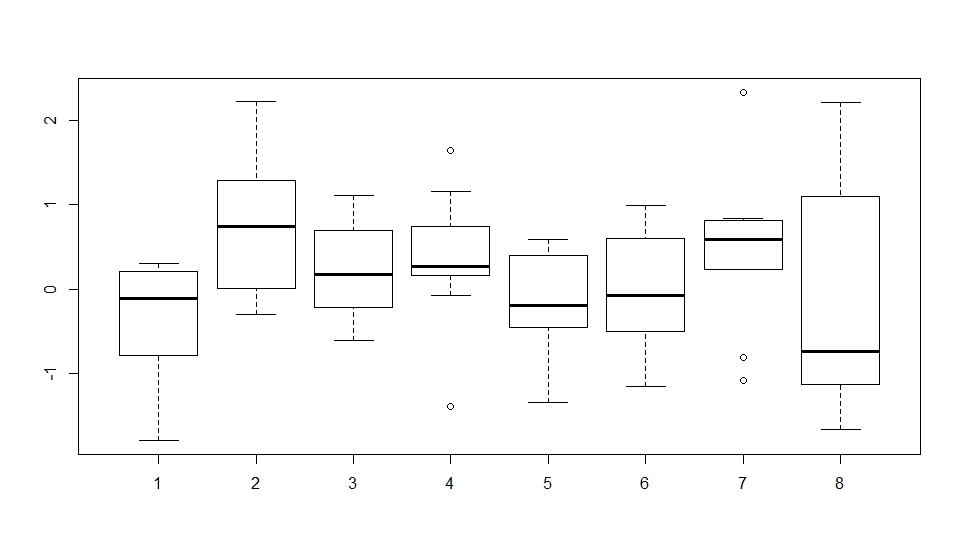
\includegraphics[width=8cm]{boxplot.jpeg}
\end{center}
\vspace*{-1cm}\pause
$\longrightarrow $ \textsc{Exercise 16}
\end{frame}


\begin{frame}
\frametitle{Data description}
\framesubtitle{Mean, variance, standard deviation}
\begin{description}
\item[\texttt{mean}] Calculates the mean of a vector, the mean of all
elements of a matrix, each column mean of a dataframe
\item[\texttt{sd}] Calculates the standard deviation of a mean, or the
standard deviation of each column of a matrix or dataframe
\item[\texttt{var}] Calculates the variance of a vector, or the covariance
matrix of a matrix or dataframe
\item[\texttt{na.rm}] All three functions have the option \texttt{na.rm}
(remove missings) which can be \texttt{TRUE} or \texttt{FALSE} (default)
\end{description}\pause
$\longrightarrow $ \textsc{Exercise 17}
\end{frame}


\begin{frame}
\frametitle{Data description}
\framesubtitle{Histograms}
\begin{itemize}
\item The built-in command \texttt{hist} generates a plot of the histogram
\item An improved command in the \texttt{library(MASS)} is \texttt{truehist}
\item See the help file of \texttt{truehist} for the options
\item Important options are: \texttt{xlab,ylab,xlim,ylim,main}
\item One can easily add lines and curves to the plot\newline
(with \texttt{abline} or \texttt{lines})
\end{itemize}
\end{frame}


\begin{frame}
\frametitle{Data description}
\framesubtitle{Histograms}
\begin{block}{Examples}
\texttt{library(MASS)}\newline
\texttt{x <- rnorm(2000) \# we come back to this later}\newline
\texttt{truehist(x)}\newline
\texttt{abline(v=0)}\newline
\texttt{g <- seq(-3,3,length=500)}\newline
\texttt{lines(g,dnorm(g))}
\end{block}\pause
$\longrightarrow $ \textsc{Exercise 18}
\end{frame}


\begin{frame}
\frametitle{Data description}
\framesubtitle{Contingency table}
\begin{itemize}
\item Contingency tables are multivariate frequency tables
\item The command \texttt{table} can tabulate multivariate data
\item If there are more than two dimensions, one can display
the tables either as arrays or as flat tables
\item One can use the \texttt{apply} command to compute marginal
distributions
\end{itemize}
\end{frame}


\begin{frame}
\frametitle{Data description}
\framesubtitle{Contingency table}
\begin{block}{Examples}
\texttt{data(UCBAdmissions)}\newline
\texttt{UCBAdmissions}\newline
\texttt{ftable(UCBAdmissions)}\newline
\texttt{ftable(UCBAdmissions,row.vars=c("Dept","Gender"))}\newline
\texttt{plot(UCBAdmissions)}\newline
\texttt{apply(UCBAdmissions,c(1,2),sum)}
\end{block}
\end{frame}


\begin{frame}
\frametitle{Data description}
\framesubtitle{Covariance}
\begin{itemize}
\item If there are two vectors $x$ and $y$ of the same length $n$, then 
\texttt{cov(x,y)} or \texttt{var(x,y)} compute the covariance%
\begin{equation*}
\frac{1}{n-1}\sum_{i=1}^{n}\left( x_{i}-\bar{x}\right) \left( y_{i}-\bar{y}%
\right)
\end{equation*}
\item If $x$ is a $\left( n,m\right) $-matrix or dataframe, then \texttt{cov(x)} or \texttt{var(x)} compute the covariance matrix of its columns
\item If missing values exist, one can specify which observations should be
included (option \texttt{use})
\end{itemize}
\end{frame}


\begin{frame}
\frametitle{Data description}
\framesubtitle{Correlation}
\begin{itemize}
\item If there are two vectors $x$ and $y$ of the same length $n$, then 
\texttt{cor(x,y)} computes the correlation coefficient (Bravais-Pearson)
\item If $x$ is a $\left( n,m\right) $-matrix or dataframe, then \texttt{cor(x)} computes the correlation matrix of its columns
\item If missing values exist, one can specify which observations should be
included (option \texttt{use})
\item Use the option \texttt{method} to compute Spearman's or Kendall's
correlation coefficients
\end{itemize}\pause
$\longrightarrow $ \textsc{Exercise 19}
\end{frame}


\section{Programming}


\begin{frame}[fragile]
\frametitle{Programming}
\framesubtitle{Loops}
\begin{itemize}
\item If the same commands should be executed for different values of some
variable, loops are useful
\item There are three kinds of loops: \texttt{for}, \texttt{while}, \texttt{repeat}
\item By far the most important loop is the \texttt{for}-loop
\item General syntax:
\end{itemize}
\begin{verbatim}
    for([var] in vector) {
        [commands]
    }
\end{verbatim}
\begin{itemize}
\item The commands are executed for each value of \texttt{vector}
\end{itemize}
\end{frame}


\begin{frame}
\frametitle{Programming}
\framesubtitle{Loops}
\begin{block}{Example}
\texttt{z <- rep(NA,10)}

\texttt{for(i in 1:10) \{}

\quad \quad \texttt{z[i] <- i\symbol{94}2}

\texttt{\}}

\texttt{print(z)}
\end{block}
\end{frame}


\begin{frame}
\frametitle{Programming}
\framesubtitle{Loops}
\begin{itemize}
\item Syntax of the \texttt{while}-loop:
\end{itemize}
\begin{center}
\texttt{while([condition]) \{[commands]\}}
\end{center}
\begin{itemize}
\item Syntax of the \texttt{repeat}-loop:
\end{itemize}
\begin{center}
\texttt{repeat \{[commands]\}}
\end{center}
\begin{itemize}
\item The \texttt{repeat}-loop does never stop but can be left using the
command \texttt{break}
\end{itemize}
\end{frame}


\begin{frame}[fragile]
\frametitle{Programming}
\framesubtitle{Conditions}
Syntax of the \texttt{if}-command
\begin{verbatim}
    if([condition]) {
       [commands]
    }
\end{verbatim}
\begin{itemize}
\item The condition must not be a vector
(else only its first element is used)
\item If there is just a single command, the brackets can be omitted
\item The opening curly bracket must appear in the same line as the \texttt{%
if}-command
\item It is possible to add \texttt{else \{[commands]\}}
\end{itemize}
\end{frame}


\begin{frame}
\frametitle{Programming}
\framesubtitle{Conditions}
\begin{itemize}
\item The function \texttt{ifelse} can be used for multiple conditions
\item Syntax of the \texttt{ifelse}-function
\end{itemize}
\begin{center}
\texttt{x <- ifelse([logical vector],a,b)}
\end{center}
\begin{itemize}
\item Then \texttt{x} is a vector of the same length as \texttt{[logical
vector]}
\item The elements of \texttt{x} are taken either from \texttt{a} or from 
\texttt{b}
\item The value vectors \texttt{a} and \texttt{b} can be scalars
\end{itemize}\pause
$\longrightarrow $ \textsc{Exercise 20}
\end{frame}


\section{Random numbers}


\begin{frame}
\frametitle{Random numbers}
\framesubtitle{Standard distributions}
\begin{itemize}
\item A large number of standard distributions is implemented in R
\item There is a common syntax for cdfs, density functions, quantile
functions, and random number generation:
\begin{description}
\item[\texttt{pNAME(x,pars)}] cumulative distribution function at $x$
\item[\texttt{dNAME(x,pars)}] density (or probability) function at $x$
\item[\texttt{qNAME(p,pars)}] quantile function at $p$
\item[\texttt{rNAME(n,pars)}] generate $n$ random draws
\end{description}
\item Here \texttt{NAME} is the abbreviated name of the distribution and 
\texttt{pars} are its parameters
\end{itemize}
\end{frame}


\begin{frame}
\frametitle{Random numbers}
\framesubtitle{Standard distributions}
Some continuous distribution names:
\begin{description}
\item[\texttt{norm}] normal
\item[\texttt{unif}] uniform
\item[\texttt{lnorm}] log-normal
\item[\texttt{exp}] exponential
\item[\texttt{t}] $t$-distribution
\item[\texttt{chisq}] $\chi ^{2}$-distribution
\item[\texttt{F}] $F$-distribution
\end{description}
\end{frame}


\begin{frame}
\frametitle{Random numbers}
\framesubtitle{Standard distributions}
Some discrete distribution names:
\begin{description}
\item[\texttt{binom}] binomial
\item[\texttt{pois}] Poisson
\item[\texttt{geom}] geometric
\item[\texttt{hyper}] hyper-geometric
\item[\texttt{nbinom}] negative binomial
\item[\texttt{multinom}] multinomial
\end{description}
\end{frame}


\begin{frame}
\frametitle{Random numbers}
\framesubtitle{Standard distributions}
\begin{itemize}
\item Define a vector $x$ on an appropriate grid $[a,b]$
\item Plots of cdf and density functions:
\end{itemize}
\begin{center}
\texttt{plot(x,pNAME(x,pars))}

\texttt{plot(x,dNAME(x,pars))}
\end{center}
\begin{itemize}
\item Define a grid vector $p$ on $[0,1]$; plot of quantile function:
\end{itemize}
\begin{center}
\texttt{plot(x,qNAME(p,pars))}
\end{center}\pause
$\longrightarrow $ \textsc{Exercise 21}
\end{frame}


\begin{frame}
\frametitle{Random numbers}
\framesubtitle{Simulations}
\begin{itemize}
\item Simulation: Evaluate many randomly generated \textquotedblleft
scenarios\textquotedblright\ (replications)
\item Standard steps:
\begin{enumerate}
\item Choose the number of replications $R$
\item Initialize an empty vector $Z$ of length $R$
\item Write a \texttt{for}-loop, e.g. over $r=1,\ldots ,R$
\item For each $r$, generate a random scenario, evaluate it, and save the result in $Z[r]$
\item After the loop, report (or plot) the result vector $Z$
\end{enumerate}
\end{itemize}
\end{frame}


\begin{frame}
\frametitle{Random numbers}
\framesubtitle{Simulations}
\begin{block}{Example}
Simulate the distribution of the moment estimator of the exponential
distribution\bigskip

\texttt{R <- 10000}

\texttt{Z <- rep(NA,R)}

\texttt{for(r in 1:R) \{}

\quad \texttt{x <- rexp(n=10,rate=0.5)}

\quad \texttt{Z[r] <- 1/mean(x)}

\texttt{\}}

\texttt{truehist(Z)}

\texttt{abline(v=2,col="red")}
\end{block}
\end{frame}


\begin{frame}
\frametitle{Random numbers}
\framesubtitle{Simulations}

\begin{block}{Example}
Simulate the distribution of the maximum of a Wiener process on the interval 
$[0,1]$\bigskip

\texttt{R <- 10000}

\texttt{N <- 500}

\texttt{Z <- rep(NA,R)}

\texttt{for(r in 1:R) \{}

\quad \texttt{x <- cumsum(rnorm(N,mean=0,sd=sqrt(1/N)))}

\quad \texttt{Z[r] <- max(x)}

\texttt{\}}

\texttt{truehist(Z)}
\end{block}\pause
$\longrightarrow $ \textsc{Exercise 22}
\end{frame}


\section{Linear regressions}
\begin{frame}
\frametitle{Linear regression}
\framesubtitle{Multiple linear regression}
\begin{itemize}
\item Consider the linear regression model%
\begin{equation*}
y_{t}=\alpha +\beta _{1}x_{1t}+\ldots +\beta _{K}x_{Kt}+u_{t}
\end{equation*}%
for $t=1,\ldots ,T$ with independent $u_{t}\sim N(0,\sigma ^{2})$
\item Matrix notation
\begin{equation*}
y=X\beta +u,\qquad u\sim N(0,\sigma ^{2}I)
\end{equation*}
\item OLS estimator
\begin{equation*}
\hat{\beta}=\left( X^{\prime }X\right) ^{-1}X^{\prime }y
\end{equation*}
\end{itemize}
\end{frame}


\begin{frame}
\frametitle{Linear regression}
\framesubtitle{Multiple linear regression}
\begin{itemize}
\item The general syntax of regression models is rather idiosyncratic:
\end{itemize}
\begin{center}
\texttt{a <- lm(formula)}
\end{center}
\begin{itemize}
\item Basic \textquotedblleft formula\textquotedblright\ syntax
\end{itemize}
\begin{center}
\texttt{y \symbol{126} x1 + x2 + \ldots\ + xK}
\end{center}
\begin{itemize}
\item Endogenous variable is on the left of \texttt{\symbol{126}}; exogenous
variables are on the right of \texttt{\symbol{126}}, separated by \texttt{+}
\end{itemize}
\end{frame}


\begin{frame}
\frametitle{Linear regression}
\framesubtitle{Multiple linear regression}
\begin{block}{Example}
\texttt{library(foreign)}

\texttt{x <- read.dta("wave2009.dta")}

\texttt{attach(x)}

\texttt{regr1 <- lm(satisfaction\symbol{126}age+netincome+children)}

\texttt{regr1}

\texttt{summary(regr1)}

\texttt{names(regr1)}
\end{block}
\end{frame}


\begin{frame}
\frametitle{Linear regression}
\framesubtitle{Multiple linear regression}
\begin{itemize}
\item The \texttt{lm}-object is a list containing:
\begin{enumerate}
\item The estimated coefficients $\hat{\beta}$
\item The residuals $\hat{u}_{t}$
\item The fitted values $\hat{y}_{t}$
\item Some other things
\end{enumerate}
\item If \texttt{a} is an \texttt{lm}-object one can access its elements
using\newline
\texttt{coefficients(a)}, \texttt{residuals(a)}, \texttt{fitted.values(a)}
\item Alternatively, one can use the \texttt{\$}-operator: \texttt{%
a\$coefficients}, \texttt{a\$residuals}, \texttt{a\$fitted.values}
\end{itemize}
\end{frame}


\begin{frame}
\frametitle{Linear regression}
\framesubtitle{Multiple linear regression}
Extensions (I):
\begin{itemize}
\item An intercept is added automatically but can be removed: \texttt{lm(y\symbol{126}x1+x2-1)}
\item If the variables are organized in an unattached dataframe \texttt{x}, 
\newline
one can use the syntax: \texttt{lm(formula,data=x)}
\item The formula may contain mathematical functions, e.g. \texttt{lm(log(y)%
\symbol{126}log(x1))}
\item \textbf{Attention}: Squares, sums and differences are not allowed!
\item Use the function \texttt{I()} for squares, sums and differences
\end{itemize}
\end{frame}


\begin{frame}
\frametitle{Linear regression}
\framesubtitle{Multiple linear regression}
Extensions (II):
\begin{itemize}
\item Syntax for interaction terms
\end{itemize}
\begin{center}
\texttt{a <- lm(y \symbol{126} x1 + x2 + x1:x2)}
\end{center}
\begin{itemize}
\item Abbreviation: \texttt{a <- lm(y \symbol{126} x1*x2)}
\item Weights can be added using the option \texttt{weights}
\item One can select a subset of observations using the option \texttt{subset%
}
\end{itemize}
\end{frame}


\begin{frame}
\frametitle{Linear regression}
\framesubtitle{Multiple linear regression}
Extensions (III):
\begin{itemize}
\item The \texttt{lm}-object can be used to add a regression line to a plot:
\newline
\texttt{regr <- lm(y\symbol{126}x)}\newline
\texttt{plot(x,y)}\newline
\texttt{abline(regr)}
\item The \texttt{lm}-object can be used for forecasting:\newline
\texttt{regr <- lm(y\symbol{126}x1+x2)}\newline
\texttt{xn <- data.frame(x1=c(...),x2=c(...))}\newline
\texttt{predict(regr,newdata=xn,se.fit=TRUE)}
\end{itemize}
\end{frame}


\begin{frame}
\frametitle{Linear regression}
\framesubtitle{Multiple linear regression}
Extensions (IV):
\begin{itemize}
\item Heteroskedasticity consistent standard errors are not reported by default
\item The package \texttt{sandwich} supplies functions for robust standard
errors (the package \texttt{sandwich} is included in the package \texttt{AER})
\item The syntax for robust standard errors is
\end{itemize}
\begin{center}
\texttt{coeftest(regr,vcov=vcovHC)}
\end{center}
\end{frame}


\begin{frame}
\frametitle{Linear regression}
\framesubtitle{Multiple linear regression}
\begin{block}{Example}
\texttt{regr2 <- lm(satisfaction\symbol{126}age+netincome,data=x)}

\texttt{regr3 <- lm(satisfaction\symbol{126}age+I(age\symbol{94}2))}

\texttt{regr4 <- lm(satisfaction\symbol{126}log(netincome))}

\texttt{regr5 <- lm(satisfaction\symbol{126}gender*marital)}

\texttt{z <- gender=="Female"}

\texttt{regr6 <- lm(satisfaction\symbol{126}log(netincome),subset=z)}

\texttt{coeftest(regr6,vcovHC)}

\end{block}\pause
$\longrightarrow $ \textsc{Exercise 23}
\end{frame}

\section{Numerical optimisation}


\begin{frame}
\frametitle{Numerical optimisation}
\framesubtitle{Univariate optimisation}
\begin{itemize}
\item In R, optimisation is minimisation
\item To maximise a function $f(x)$, minimise $-f(x)$
\item Suppose $f(x)$ has a minimum in the interval $[a,b]$
\item The minimum is at $x^{\ast }$ with $f(x^{\ast })\leq f(x)$ for all $x\in \lbrack a,b]$
\item The univariate optimisation command is
\end{itemize}
\begin{center}
\texttt{a <- optimize(f,interval=c(a,b))}
\end{center}
\begin{itemize}
\item The command returns a list with two components: \newline
\texttt{a\$minimum} ($x^{\ast }$), \texttt{a\$objective} ($f(x^{\ast })$)
\end{itemize}
\end{frame}


\begin{frame}
\frametitle{Numerical optimisation}
\framesubtitle{Univariate optimisation}
\begin{block}{Example}
\texttt{f1 <- function(x) \{}

\quad \texttt{a <- 1/exp(-(x-3)\symbol{94}2)}

\quad \texttt{return(a)}

\texttt{\}}

\texttt{m1 <- optimize(f1,interval=c(-5,5))}

\texttt{print(m1)}

\texttt{m2 <- optimize(f1,interval=c(-2,2))}

\texttt{print(m2)}
\end{block}
\end{frame}


\begin{frame}
\frametitle{Numerical optimisation}
\framesubtitle{Multivariate optimisation}
\begin{itemize}
\item Consider a scalar-valued function $f(x_{1},\ldots ,x_{n})$
\item The multivariate optimisation command is
\end{itemize}
\begin{center}
\texttt{a <- optim(x0,f)}
\end{center}
\begin{itemize}
\item The algorithm starts at $x_{0}=(x_{01},\ldots ,x_{0n})$ and searches the minimum iteratively
\item The more dimensions $n$, the harder it is to find the optimum
\item Attention: The optimum might be a local optimum!
\end{itemize}
\end{frame}


\begin{frame}
\frametitle{Numerical optimisation}
\framesubtitle{Multivariate optimisation}
Remarks:
\begin{itemize}
\item The function \texttt{f} can have more arguments than \texttt{x}, e.g. \texttt{f(x,a)}
\item Additional arguments can be supplied via the \texttt{optim} command,
e.g. \texttt{optim(x0,f,a=}$\mathtt{\ldots }$\texttt{)}
\item Additional options can also be set, see \texttt{?optim}
\item The numerical optimisation method can be changed by the \texttt{method}-option
\item The \texttt{L-BFGS-B} method allows to add limits (to prevent the
algorithm from wandering into \textquotedblleft forbidden
areas\textquotedblright )
\end{itemize}
\end{frame}


\begin{frame}
\frametitle{Numerical optimisation}
\framesubtitle{Multivariate optimisation}
\begin{block}{Example}
\texttt{fn <- function(x) \{}

\quad \texttt{a <- x[1]\symbol{94}2+(x[2]-2)\symbol{94}2}

\quad \texttt{return(a)}

\texttt{\}}

\texttt{m1 <- optim(c(0,0),fn)}

\texttt{print(m1)}

\texttt{m2 <- optim(c(0,0),fn,}

\quad \texttt{method="L-BFGS-B",lower=c(0,0),upper=c(0.5,1))}

\texttt{print(m2)}
\end{block}\pause
$\longrightarrow $ \textsc{Exercise 24}
\end{frame}


\section{Maximum likelihood}

\begin{frame}
\frametitle{Maximum likelihood}
\framesubtitle{Basic idea}
\begin{itemize}
\item The basic idea is very natural:
\item Choose the parameters such that the probability (likelihood) of the
observations $x_{1},\ldots ,x_{n}$ as a function of the unknown parameters $\theta _{1},\ldots ,\theta _{r}$ is maximized
\item Likelihood function
\begin{equation*}
L(\theta ;x_{1},\dots ,x_{n})=\left\{ 
\begin{array}{l}
P(X_{1}=x_{1},\ldots ,X_{n}=x_{n};\theta ) \\[3mm] 
f_{X_{1},\dots ,X_{n}}(x_{1},\dots ,x_{n};\theta )%
\end{array}%
\right.
\end{equation*}
\end{itemize}
\end{frame}


\begin{frame}
\frametitle{Maximum likelihood}
\framesubtitle{Basic idea}
\begin{itemize}
\item For simple random samples
\begin{equation*}
L(\theta ;x_{1},\dots ,x_{n})=\prod_{i=1}^{n}f_{X}(x_{i};\theta )
\end{equation*}
\item Log-likelihood function
\begin{equation*}
\ln L(\theta ;x_{1},\ldots ,x_{n})=\sum_{i=1}^{n}\ln f_{X}(X_{i};\theta )
\end{equation*}
\item Maximize the log-likelihood function $\longrightarrow $ $\hat{\theta}$
\end{itemize}
\end{frame}


\begin{frame}
\frametitle{Maximum likelihood}
\framesubtitle{Basic idea}
\begin{itemize}
\item Sometimes, one can find $\hat{\theta}$ analytically by solving%
\begin{eqnarray*}
\partial \ln L/\partial \theta _{1} &=&0 \\
&\vdots & \\
\partial \ln L/\partial \theta _{r} &=&0
\end{eqnarray*}
\item If the log-likelihood is not differentiable other maximization methods
must be used, e.g. numerical maximization of the log-likelihood
\end{itemize}
\end{frame}


\begin{frame}
\frametitle{Maximum likelihood}
\framesubtitle{Properties of ML estimators}
\begin{enumerate}
\item Equivariance: If $\hat{\theta}$ is the ML estimator for $\theta $,
then $g(\hat{\theta})$ is the ML estimator for $g(\theta )$
\item Consistency: $ \text{plim\;} \hat{\theta}_{n}\mathbf{=}\theta $
\item Asymptotic normality
\item Asymptotic efficiency
\item Computability (analytical or numerical); the covariance matrix of the
estimator is a by-product of the numerical method
\end{enumerate}
\end{frame}


\begin{frame}
\frametitle{Maximum likelihood}
\framesubtitle{Properties of ML estimators}
\begin{block}{Example}
Numerical estimation of the parameters of $N(\mu ,\sigma ^{2})\medskip $

\texttt{negloglik <- function(theta,x) \{}

\quad \texttt{mu <- theta[1]}

\quad \texttt{sigma <- theta[2]}

\quad \texttt{return(-sum(log(dnorm(x,mu,sigma))))}

\texttt{\}}

\texttt{dat <- rnorm(n=50,mean=5,sd=3) \# generate a sample}

\texttt{ML <- optim(c(0,1),negloglik,x=dat)}

\texttt{print(ML)}
\end{block}\pause
$\longrightarrow $ \textsc{Exercise 25}
\end{frame}


\section{Time Series}
\begin{frame}	
	\frametitle{Time series}	
	\framesubtitle{Packages}	
	Useful packages for time series analysis include:	
	\begin{itemize}
		\item \texttt{tseries}		
		\item \texttt{fGarch} (also installs \texttt{timeDate}, \texttt{timeSeries}, \texttt{fBasics})
		\item \texttt{vars}		
		\item \texttt{zoo}
	\end{itemize}	
	\medskip See Task View \textquotedblleft TimeSeries\textquotedblright\ on
	the CRAN site for many more\newline
	time series packages.
\end{frame}


\begin{frame}
	\frametitle{Time series}	
	\framesubtitle{Date and time classes}	
	\begin{itemize}
		\item The class \texttt{Date} represents calendar dates (days)		
		\item Generate a single date, 
		\begin{equation*}
		\text{\texttt{as.Date("YYYY-MM-DD")}}
		\end{equation*}		
		\item Generate a vector of dates,
		\begin{equation*}
		\text{\texttt{seq(date1,date2,by="unit")}}
		\end{equation*}
		where \texttt{unit} can be \texttt{days}, \texttt{weeks}, \texttt{months}, 
		\texttt{years} \newline
		(or even \texttt{4 days}, \texttt{2 months} etc.)
	\end{itemize}
\end{frame}


\begin{frame}	
	\frametitle{Time series}	
	\framesubtitle{Date and time classes}	
	\begin{itemize}
		\item The class \texttt{POSIXt} (\texttt{POSIXct}, \texttt{POSIXlt})
		represents calendar dates and times		
		\item Generate a single date,
		\begin{equation*}
		\text{\texttt{strptime("datestring","format")}}
		\end{equation*}
		where \texttt{datestring} describes the date and time, and \texttt{format}
		explains the format		
		\item Example:\newline
		\texttt{strptime("2011/12/31-23:59:59","\%Y/\%m/\%d-\%H:\%M:\%S")}
	\end{itemize}
\end{frame}


\begin{frame}	
	\frametitle{Time series}	
	\framesubtitle{Date and time classes}	
	\begin{itemize}
		\item Generate a vector of dates,
		\begin{equation*}
		\text{\texttt{seq(date1,date2,by="units")}}
		\end{equation*}%
		where \texttt{units} can be \texttt{years}, \texttt{months}, \texttt{weeks}, 
		\texttt{days}, \texttt{hours}, \texttt{mins}, \texttt{secs} (also \texttt{20
			mins}, etc.)		
		\item Date classes can be converted by \texttt{as.Date}, \texttt{as.POSIXlt}%
		, etc.		
		\item Useful functions for dates include \texttt{diff}, \texttt{difftime}, 
		\texttt{"-"}, \texttt{weekdays}, \texttt{months}, \texttt{quarters}		
		\item Logical operators, e.g. \texttt{date1>date2}, \texttt{%
			date3==date4}
	\end{itemize}
\end{frame}


\begin{frame}
	\frametitle{Time series}	
	\framesubtitle{Date and time classes}	
	\begin{block}{Examples}
		\texttt{d1 <- as.Date("2012-01-01")}
				
		\texttt{d2 <- as.Date("2012-01-31")}
		
		\texttt{d2-d1}
		
		\texttt{difftime(d2,d1,units="hours")}
		
		\texttt{dd <- seq(d1,d2,by="days")}
		
		\texttt{print(dd)}
		
		\texttt{plot(dd,rnorm(31),type="o")}
		
		\texttt{weekdays(dd)}
		
		\texttt{dd > as.Date("2012-01-15")}
	\end{block}
\end{frame}


\begin{frame}
	\frametitle{Time series}	
	\framesubtitle{Date and time classes}	
	\begin{block}{Examples}
		\texttt{f <- "\%Y-\%m-\%d \%H:\%M:\%S"}
		
		\texttt{d1 <- strptime("2012-01-01 15:00:00",f)}
		
		\texttt{d2 <- strptime("2012-01-02 16:00:00",f)}
		
		\texttt{difftime(d2,d1,units="hours")}
		
		\texttt{dd <- seq(d1,d2,by="30 mins")}
		
		\texttt{print(dd)}
		
		\texttt{plot(dd,rnorm(51),type="o")}
		
		\texttt{weekdays(dd)}
		
		\texttt{dd > strptime("2012-01-01 19:00:00",f)}
	\end{block}\pause
	$\longrightarrow $ \textsc{Exercise 26}
\end{frame}


\begin{frame}
	\frametitle{Time series}	
	\framesubtitle{Time series classes}	
	\begin{itemize}
		\item The elementary time series class is \texttt{ts}		
		\item A \texttt{ts}-object is either a vector (univariate time series) or a
		matrix (multivariate time series) plus attributes		
		\begin{enumerate}
			\item start			
			\item end			
			\item frequency
		\end{enumerate}		
		\item The attributes of a time series object can be read by the function 
		\texttt{tsp} (\textbf{t}ime \textbf{s}eries \textbf{p}roperties)		
		\item Most time series functions also accept vectors (or matrices) as inputs
	\end{itemize}
\end{frame}


\begin{frame}
	\frametitle{Time series}	
	\framesubtitle{Time series classes}	
	\begin{block}{Examples}
		\texttt{x <- cumsum(rnorm(30))}	
		
		\texttt{y <- ts(x,start=c(2002,2),frequency=4)}
		
		\texttt{print(y)}
		
		\texttt{plot(y)}
		
		\texttt{lag(y)}
		
		\texttt{lag(y,-1)}
		
		\texttt{diff(y)}
		
		\texttt{window(y,start=c(2003,1),end=c(2008,4))}
	\end{block}	
\end{frame}


\begin{frame}
	\frametitle{Time series}	
	\framesubtitle{Time series classes}	
	\begin{itemize}
		\item The class \texttt{ts} is not very flexible and mainly meant for
		quarterly or monthly data		
		\item The class \texttt{zoo} is more flexible and allows irregular time
		series		
		\item A zoo object is a vector or matrix plus index vector as an attribute
		giving time points (or periods)		
		\item The index vector can be of (almost) any class		
		\item Suitable classes are: \texttt{vector}, \texttt{Date}, \texttt{POSIXlt}
	\end{itemize}
\end{frame}


\begin{frame}
	\frametitle{Time series}	
	\framesubtitle{Time series classes}	
	\begin{block}{Examples}
		\texttt{x <- cumsum(rnorm(30))}
			
		\texttt{y <- zoo(x,order.by=1981:2010)}
		
		\texttt{print(y)}
		
		\texttt{print(index(y))}
		
		\texttt{plot(y)}
		
		\texttt{lines(lag(y,-1),col="red")}
		
		\texttt{lines(rollmean(y,k=4),col="blue")}
		
		\texttt{diff(y)}
		
		\texttt{window(y,start=1985,end=2000)}
	\end{block}
\end{frame}


\begin{frame}
	\frametitle{Time series}	
	\framesubtitle{Time series: ACF}	
	\begin{itemize}
		\item One of the most important statistics about a time series is the
		autocorrelation function
		\begin{equation*}
		\hat{\rho}(s)=\frac{\sum_{t=s+1}^{T}\left( X_{t}-\bar{X}\right) \left(
			X_{t-s}-\bar{X}\right) }{\sum_{t=1}^{T}\left( X_{t}-\bar{X}\right) ^{2}}
		\end{equation*}		
		\item The function \texttt{acf} computes (and plots) the autocorrelation
		function for $s=0,1,2,\ldots ,$lag.max		
		\item It can also be used to compute autocovariance and partial
		autocorrelations
	\end{itemize}\pause
	$\longrightarrow $ \textsc{Exercise 27}
\end{frame}


\begin{frame}
	\frametitle{Time series}	
	\framesubtitle{Model estimation: AR(p)}	
	\begin{itemize}
		\item $AR(p)$, autoregressive process of order $p$,
		\begin{equation*}
		\left( X_{t}-\mu \right) =\alpha _{1}\left( X_{t-1}-\mu \right) +\ldots
		+\alpha _{p}\left( X_{t-p}-\mu \right) +\varepsilon _{t}
		\end{equation*}%
		where $\varepsilon _{t}$ is a white noise process with variance $\sigma
		_{\varepsilon }^{2}$		
		\item $AR(p)$ models can be estimated by
		\begin{equation*}
		\text{\texttt{ar(x,order.max=p,aic=F)}}
		\end{equation*}		
		\item The lag order $p$ can be given or automatically determined by the
		Akaike information criterion (set \texttt{aic=TRUE})
	\end{itemize}
\end{frame}


\begin{frame}
	\frametitle{Time series}
	\framesubtitle{Model estimation: ARIMA(p,d,q)}	
	\begin{itemize}
		\item $ARIMA(p,d,q)$, autoregressive integrated moving average process of
		order $p$, $d$, $q$%
		\begin{eqnarray*}
			\left( \Delta^d X_{t}-\mu \right)  &=&\alpha _{1}\left( \Delta^d X_{t-1}-\mu \right) +\ldots
			+\alpha _{p}\left( \Delta^d X_{t-p}-\mu \right)  \\
			&&+\varepsilon _{t}+\theta _{1}\varepsilon _{t-1}+\ldots +\theta
			_{q}\varepsilon _{t-q}
		\end{eqnarray*}%
		where $\varepsilon _{t}$ is a white noise process with variance $\sigma
		_{\varepsilon }^{2}$ and $\Delta^d$ is the difference operator taken $d$ times. 
		\item $ARIMA$ models can be estimated by 
	\end{itemize}	
	\begin{center}
		\texttt{arima(x,order=c(p,d,q))}
	\end{center}
\end{frame}


\begin{frame}
	\frametitle{Time series}	
	\framesubtitle{Model estimation: GARCH(p,q)}	
	\begin{itemize}
		\item $GARCH(p,q)$, generalized autoregressive conditional heteroskedastic
		process of order $p,q$%
		\begin{eqnarray*}
			X_{t} &=&\sigma _{t}\cdot \varepsilon _{t} \\
			\varepsilon _{t} &\sim &N(0,1) \\
			\sigma _{t}^{2} &=&\alpha _{0}+\alpha _{1}X_{t-1}^{2}+\ldots +\alpha
			_{p}X_{t-p}^{2} \\
			&&+\beta _{1}\sigma _{t-1}^{2}+\ldots +\beta _{q}\sigma _{t-q}^{2}
		\end{eqnarray*}		
		\item Often, there is also a mean equation for $X_{t}$, e.g.%
		\begin{equation*}
		X_{t}=\mu +\gamma _{1}Z_{1t}+\ldots +\gamma _{K}Z_{Kt}+\sigma
		_{t}\varepsilon _{t}
		\end{equation*}
	\end{itemize}
\end{frame}


\begin{frame}	
	\frametitle{Time series}	
	\framesubtitle{Model estimation: GARCH(p,q)}	
	\begin{itemize}
		\item $GARCH$ models without mean equation can be estimated by%
		\begin{equation*}
		\text{\texttt{garch(x,order=c(p,q))}}
		\end{equation*}%
		of the \texttt{tseries} package		
		\item To estimate more complex $GARCH$ models, use the command%
		\begin{equation*}
		\text{\texttt{garchFit}}
		\end{equation*}%
		of the \texttt{fGarch} package, see \texttt{?garchFit}
	\end{itemize}
\end{frame}


\begin{frame}	
	\frametitle{Time series}	
	\framesubtitle{Model estimation: VAR(p)}	
	\begin{itemize}
		\item $VAR(p)$, multivariate vector autoregressive models of order $p$ can
		be estimated by%
		\begin{equation*}
		\text{\texttt{VAR(x,p)}}
		\end{equation*}%
		where \texttt{x} is a multivariate time series object (or a matrix) \newline
		and \texttt{p} is a scalar		
		\item Package \texttt{vars}		
		\item The return object is of class \texttt{varest} and can be used for
		forecasting and impuls response functions
	\end{itemize}
\end{frame}


\begin{frame}
	\frametitle{Time series}	
	\framesubtitle{Unit root tests}	
	\begin{itemize}
		\item The standard unit root test is the augmented Dickey-Fuller test (ADF
		test)		
		\item Test of $H_{0}:\rho =0$ in the regression
		\begin{equation*}
		\Delta X_{t}=\alpha +\delta t+\rho X_{t-1}+\sum_{j=1}^{k}\phi _{j}\Delta
		X_{t-j}+\varepsilon _{t}
		\end{equation*}		
		\item Function \texttt{adf.test} in the \texttt{tseries} package		
		\item Other tests are also implemented, e.g. Phillips-Perron (\texttt{pp.test}) and KPSS (\texttt{kpss.test})
	\end{itemize}\pause
	$\longrightarrow $ \textsc{Exercise 28}
\end{frame}

\end{document}
